\usetikzlibrary{arrows.meta}
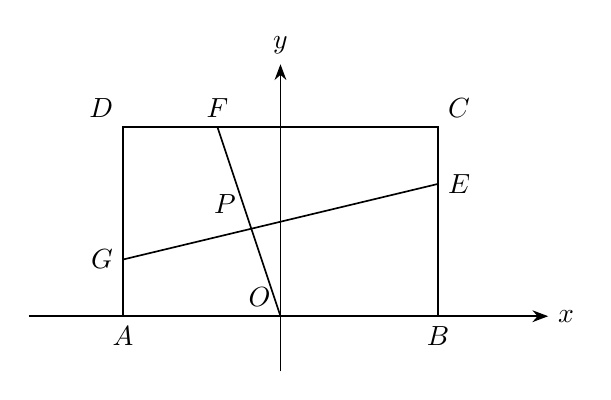
\begin{tikzpicture}[x=1cm,y=1cm,line width=.6pt,font=\normalsize,>=Stealth]
\coordinate (A) at (-2,0);
\coordinate (B) at (2,0);
\coordinate (O) at (0,0);
\coordinate (D) at (-2,2.4);
\coordinate (C) at (2,2.4);
\coordinate (G) at (-2,0.72);
\coordinate (E) at (2,1.68);
\coordinate (F) at (-0.8,2.4);
\coordinate (P) at (-0.3703703703703704,1.1111111111111112);
% axes: x along AB, y up through O; tips clear of rectangle
\draw[->] (-3.2,0)--(3.4,0) node[right] {$x$};
\draw[->] (0,-0.7)--(0,3.2) node[above] {$y$};
% rectangle frame
\draw (A)--(B)--(C)--(D)--cycle;
% moving-point segments (single paths, no arrowheads)
\draw (G)--(E);
\draw (O)--(F);
% labels placed in visible whitespace, off the lines
\node[below] at (A) {$A$};
\node[below] at (B) {$B$};
\node[above left] at (O) {$O$};
\node[above left] at (D) {$D$};
\node[above right] at (C) {$C$};
\node[left] at (G) {$G$};
\node[right] at (E) {$E$};
\node[above] at (F) {$F$};
\node[above left,xshift=-2pt,yshift=2pt] at (P) {$P$};
\end{tikzpicture}
